\chapter{A new chapter}
Your second chapter probably has novel material in it. hopefully.

% Add additional \chapter{}s as necessary.

% use \cite{} to cite a reference in your bibliography file.
% use \ref{} to reference a \label{} from an equation, figure, or table.

% for sets of equations use align or gather:
%\begin{align}
%\end{align}

% for long equations, use multline.

% for figures:
\begin{figure}[ht]
\centering
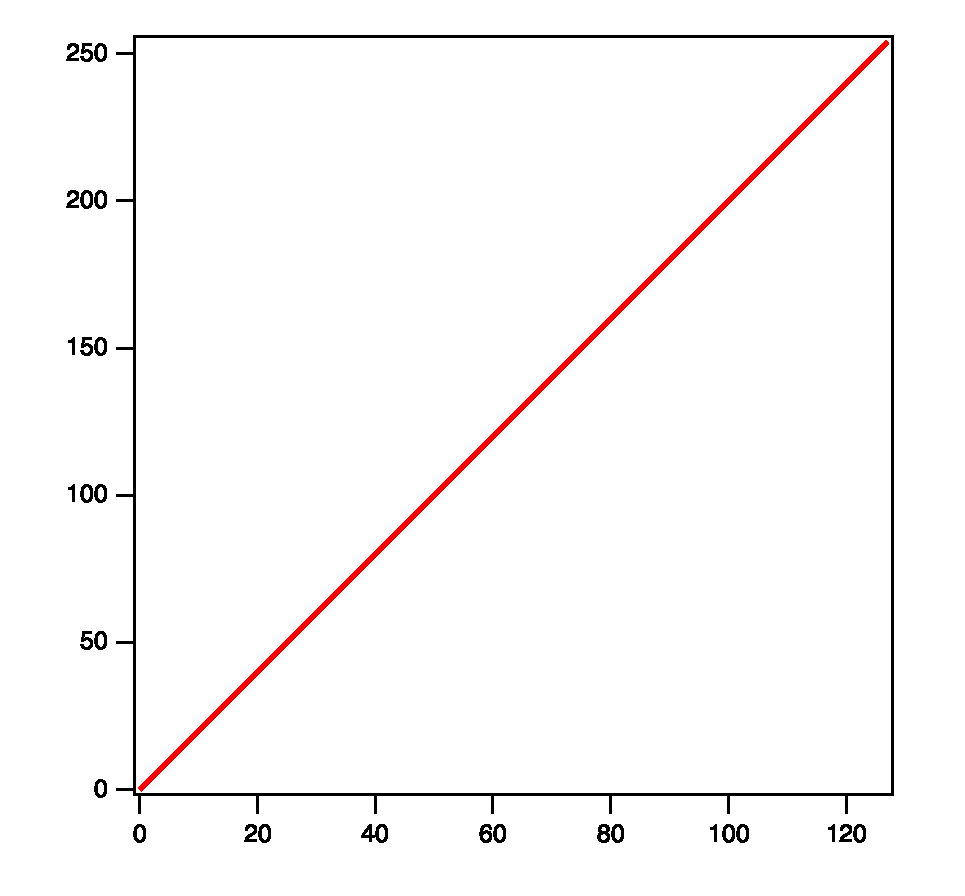
\includegraphics[width=.45\textwidth]{name_of_figure.eps}
\caption{A caption! \label{a_figure}}
\end{figure}

% for tables:
\begin{table}
\centering
\begin{tabular}{c|c|c}
 1 & 2 & 3 \\
\hline
\end{tabular}
\caption{Another caption! \label{a_table}}
\end{table}
